\documentclass[11pt]{jsk-thesis}

%レイアウト補正
%\usepackage{layout}
%\setlength \voffset {-1.0cm}
%\setlength \hoffset {-1.2cm}
%\setlength \textwidth {17cm}
%\setlength \textheight {24cm}

%パッケージ読み込み
\usepackage[dvipdfmx]{graphicx}
\usepackage[dvipdfmx]{color}
\usepackage{booktabs}
\usepackage{amsmath}
\usepackage{amssymb}
\usepackage{bm}
\usepackage{url}

%コマンド定義
%表の日付のフォントサイズ変更
\newcommand{\tdate}[1]{\scriptsize{#1}}
%単位"°"
%%\newcommand{\degree}[1]{#1^{\circ}}
%微分演算子関係
\newcommand{\dd}{\mathrm{d}}
\newcommand{\diff}[2]{\frac{\mathrm{d}#1}{\mathrm{d}#2}} %常微分
\newcommand{\diffline}[2]{\mathrm{d}#1/\mathrm{d}#2} %文章中での常微分
\newcommand{\ddiff}[3]{\frac{\mathrm{d}^#1 #2}{\mathrm{d} #3^#1}} %高階常微分
\newcommand{\ddiffline}[3]{\mathrm{d}^#1 #2/\mathrm{d} #2^#1} %文章中での高階常微分
\newcommand{\pdiff}[2]{\frac{\partial #1}{\partial #2}} %偏微分
\newcommand{\pddiff}[3]{\frac{\partial^#1 #2}{\partial #3^#1}} %高階偏微分
\newcommand{\non}[1]{#1^{*}} %無次元化変数

%関数
\newcommand{\erf}{\mathrm{erf}}

%その他
\newcommand{\myfig}[5]{
  \begin{figure}[#1]%
    \begin{center}%
      \includegraphics[width=#2]{#3}%
      \caption{#4}%
      \label{fig:#5}%
    \end{center}%
  \end{figure}%
}
%% \newcommand{\figref}[1]{Fig.\ref{fig:#1}}
%% \newcommand{\seclabel}[1]{\label{sec:#1}}
%% \newcommand{\secref}[1]{第{\bf\ref{sec:#1}}節}

\newcommand{\unit}[1]{\,[\mathrm{#1}]}

%見出し変更
\renewcommand{\figurename}{Fig.}
\renewcommand{\tablename}{Table}

\usepackage{ikuo}%%便利コマンド集.
\usepackage{jtygm}

\usepackage[dvipdfmx]{hyperref}  % 目次や参考文献をリンクにする。
\usepackage{pxjahyper} %% これを入れるとしおりが文字化けしない。out2uniが不要になる。
%% \hypersetup{bookmarksnumbered=true}
\hypersetup{colorlinks=true}
\hypersetup{linkcolor=black}
%% \hypersetup{linkbordercolor=black}
\hypersetup{urlcolor=black}
%% \hypersetup{urlbordercolor=black}
\hypersetup{citecolor=black}
%% \hypersetup{citebordercolor=black}

\usepackage{url} % \url のために必要。パッケージが無い人は探して入れる。
%% \url{http://nile.ulis.ac.jp/~yuka/}のようにして使う。

\newcommand{\FIGDIR}{./fig}        %図を置くディレクトリを指定する


\date{令和3年度修士論文}
\title{四肢から独立した翼で羽ばたいて飛ぶ感覚の提示 Presenting the sensation of flying with flapping virtual wings independent of the limbs}
\author{指導教員 水内 郁夫 教授 \\
\ \\
東京農工大学 \\
工学部 機械システム工学科 \\
\ \\
令和2年度入学\\
20643010\\
{\bf 遠藤 健}}

\begin{document}
\setlength{\baselineskip}{20pt}
\maketitle
\tableofcontents

%%各章は別ファイルにして以下にinculudeすると良い.
% \chapter[長いタイトルを改行する場合はこのようにしましょう(見出し用)]%
        {長いタイトルを改行する場合は\\このようにしましょう}

        \figb{photo.jpg}{width=0.75\hsize}{ある日の研究室}%

        \fig{fig1.eps}{width=.9\hsize}{何かの図}%

        \section{研究の背景と目的}
        \seclabel{intro}

        研究室が散らかっている(\figref{photo.jpg}参照)ので、片付けるロボットが欲
        しい。

        この図(\figref{fig1.eps})はなんだろう?

        \secref{intro}ではほげほげ。

        こういう研究\cite{Ikuo:doctor}もありました。

        ああいう研究\cite{Hondo:JRSJ2011}もありました。

        bibファイルでは、著者名(author=)は、
        「苗字 名前 and 苗字 名前 and 苗字 名前」
        のようにするんですよ\cite{Mizuuchi:RSJ2015-baneoid}。
        間は全部半角スペースですよ。

        \section{従来研究}

        \begin{table}[tb]
          \tablabel{hogehoge}
          \begin{center}
            \caption{試しに作った表}
            \begin{tabular}{l|c|r|r}
              \hline
              項目 & 数値 & コメント & 備考 \\
              \hline
              a & 10.0 & こめんとしがたい & どうすべ?\\
              b & 20.0 & こめんとしがたい & どうすべ?\\
              c & -100.0 & こめんとしがたい & どうすべ?\\
              \hline
            \end{tabular}
          \end{center}
        \end{table}

        \tabref{hogehoge}に、何かの表を示す。

        \section{本論文の構成}

\chapter[ロボメック2021の内容]%
        {ロボメック2021の内容}
    
\section{緒言}

\fig{WingMan.png}{width=1\hsize}{Flying with flapping virtual wings independent of the limbs}

\fig{How2present_the_feeling_of_flapping_eng.pdf}{width=1\hsize}{Research concept}

ヒトは古くから空を飛ぶことに憧れを抱いている.実際に飛ぶことにはリスクやコストが伴うが,VR装置を使用することで簡単に飛行体験が可能である.
\figref{WingMan.png}は,四肢から独立した翼で羽ばたいて飛ぶ様子を示した物である.
本研究では,
VR装置を用いて\figref{WingMan.png}のように羽ばたいて飛ぶ感覚の提示手法を提案する.

    \subsection{浮遊感・飛ぶ感覚・羽ばたいて飛ぶ感覚の定義}
    本研究では「羽ばたいて飛ぶ感覚」を「浮遊感」,「飛ぶ感覚」を用いて次のように位置づける.
    「浮遊感」とは,空中に浮いて漂っている感覚を指す.「飛ぶ感覚」は浮遊感に空中を移動する感覚を追加したものとする.本稿で注目する「羽ばたいて飛ぶ感覚」は,飛ぶ感覚に加え,翼を羽ばたかせる感覚を追加したものである.

    \subsection{関連研究}    
    浮遊感や飛ぶ感覚を与える研究は多く行われてきた.視覚刺激をによって発生する落下感覚に関しての研究\cite{奥川夏輝2017VR空間における視覚刺激によって発生する落下感覚の分析}や身体幇助メカニズムを用いた飛行体験装置の提案\cite{鈴木拓馬2014hmd}等がある.また,飛行しているドローンを上半身のジェスチャーで制御し,ドローンからの映像をヘッドマウントディスプレイ(以下HMD)によって与えることで飛ぶ感覚を提示する研究\cite{rognon2018flyjacket}もある.

    浮遊感と飛ぶ感覚の研究に対して,鳥のように羽ばたいて飛ぶ感覚を与える研究はまだ少ない.羽ばたいて飛ぶ感覚を与える研究の例としては,飛行中の鳥の体験をすることができる装置であるBirdly\cite{rheiner2014birdly}やHypersuit\cite{hypersuit}がある.操縦装置にうつ伏せで搭乗し手と腕を用いて翼を動かしながら,鳥視点での景色の映像を提示することで,飛行中の鳥のような体験できる装置である.

    \subsection{研究目的}
    従来の羽ばたいて飛ぶ感覚を与える研究は,ヒトが鳥のように腕を動かすことによって羽ばたいて飛ぶ感覚を提示していた.しかし,大がかりな装置が必要であることや,手足の動きが制限されるといったデメリットが存在する.
    また,羽ばたいて飛ぶ感覚を与える研究において,\figref{WingMan.png}のような背中から翼が生えた生物になる感覚を提示する研究はまだ着目されていない.

    そこで四肢から独立した翼を用いて,羽ばたいて飛ぶ感覚を提示する方法を提案する.
    本研究では,
    % 大がかりな装置を使用しないこと,(核ではないので排除)
    四肢を用いずに翼を操作している感覚の提示手法とVR空間で翼に作用する力をヒトに提示する手法を考案する.
    これにより,羽ばたいて飛んでいる状態での投擲や射撃が可能となる.これらのように飛行体験中に手足を使用する新しいアプリケーションが期待できる.

    本研究では,ヒトに翼が生えている感覚を与えるために,身体像の拡張について注目をする.

    
    \subsection{身体像の拡張}
    ヒトは身体像と呼ばれる,自身の身体形状を知覚する能力を有している.それにより自己とそれ以外を区別することができる.しかし,自己以外の部分に身体像が拡張する場合がある.身体像の拡張に関する代表的な研究として,
    % 偽物の手である
    ラバーハンドをあたかも自分の手のように感じるラバーハンド錯覚についての研究がある\cite{botvinick1998rubber}.視界から隠れた本物の手と目の前にあるラバーハンドに絵筆等で2分から20分程度同期した触覚刺激を与え続けると,ラバーハンド上に触覚刺激を知覚するという錯覚現象である.
    このように提示される視覚情報と,触覚情報の位置が一致または近しければ身体像を拡張することが可能となる.
    ラバーハンド錯覚ではヒトは情報を受けとるだけであったが,ヒトから情報を送信し,それに対する返信を受け取ることで身体像の拡張をより円滑にすることができると考える.
    
    身体像の拡張には情報の双方向性が重要であることを踏まえ,本研究では\figref{How2present_the_feeling_of_flapping_eng.pdf}のような形で身体像の拡張を行う.
    ヒトから仮想翼へは,翼を動かす指令を与える.仮想翼からヒトへは,翼が生えている様子,翼を動かして飛んでいる様子,翼へ作用する空気抵抗の感覚を伝える.上記より,四肢から独立した翼で羽ばたいて飛ぶ感覚を提示する.
    
    \subsection{ヒトから仮想翼}
    まず,ヒトから仮想翼へ翼を動かす指令を与える方法について述べる.

    ヒトから仮想翼を操作する方法として,コントローラやジェスチャによる操作や,生体信号を用いることが挙げられる.
    本研究では,四肢以外で動かすことが目的なので,主に手を用いるコントローラや,手足の動きが必要となるジェスチャではなく,生体信号を用いる.また,生体信号の中でも数値の取得が容易な筋電位によって翼を操作する.

    \fig{How2present_force_applied2wings_eng.pdf}{width=1\hsize}{How to present force applied virtual wings}




   
        



\chapter[序論]%
        {序論}

        \fig{WingMan.png}{width=1\hsize}{Flying with flapping virtual wings independent of the limbs}

        ヒトは古くから空を飛ぶことに憧れを抱いている.
        これまで私たちは,飛行機やハンググライダーといった乗り物を用いることで飛行体験をしてきた.
        また,個人飛行装置\footnote{Portable Parsonal Airmobility System...ジェットパック,動力式ウイングスーツ,動力式パラフォイル(風により展開される柔軟構造を持つ翼.Ex.パラグライダーの翼)}
        のような,ウェアラブルな装置で空を飛ぶ研究も行われている\cite{gravityindustries}.
        % 実際に飛ぶことにはリスクやコストが伴うが,VR装置を使用することで簡単に飛行体験が可能である.
        しかし,実際に空を飛ぶことは墜落などのリスクや燃料といったコスト,機器を操縦するための技術が必要となる.
        VR(Virtual Reality: 仮想現実)システムを使用することで,それらリスクやコストを回避し,乗り物・ウェアラブルな装置を問わず簡単に飛行体験が可能となる.

        \figref{WingMan.png}は,四肢から独立した翼で羽ばたいて飛ぶ様子を示した図である.
        本研究では,VRシステムを用いて\figref{WingMan.png}のように,ヒトの背中から翼が生えた生物になり羽ばたいて飛ぶ感覚の提示手法を提案する.

\section{本研究での羽ばたいて飛ぶ感覚の定義}
        本論文では「浮遊感」,「飛ぶ感覚」,「羽ばたいて飛ぶ感覚」を\figref{intro-Classification_of_floating_feeling.pdf}のように位置付ける.
        \fig{intro-Classification_of_floating_feeling.pdf}{width=1\hsize}{Classification of floating feeling}

        \begin{itemize}
                \item 「浮遊感」\\
                ...空中に浮いて漂っている感覚.
                \item 「飛ぶ感覚」\\
                ...「浮遊感」に,空中を移動する感覚を追加した感覚.
                \item 「羽ばたいて飛ぶ感覚」\\
                ...「飛ぶ感覚」に,翼を羽ばたかせる感覚を追加した感覚.
        \end{itemize}

\section{研究の背景と目的}
% VRの飛ぶ研究についてもっと充実させる(分類して一気にciteする感じ)
% 身体像拡張は次章で引用

        VR装置を用いた「浮遊感」や「飛ぶ感覚」を与える研究は多く行われてきた.視覚刺激をによって発生する落下感覚に関しての研究\cite{奥川夏輝2017VR空間における視覚刺激によって発生する落下感覚の分析}や身体幇助メカニズムを用いた飛行体験装置の提案\cite{鈴木拓馬2014hmd}等がある.また,飛行しているドローンを上半身のジェスチャーで制御し,ドローンからの映像をHMD(Head Mounted Display: ヘッドマウントディスプレイ)によって与えることで飛ぶ感覚を提示する研究\cite{rognon2018flyjacket}もある.

        \fig{Birdly.jpg}{width=0.7\hsize}{System of presenting the sensation of flying with flapping wings\cite{rheiner2014birdly}}

        「羽ばたいて飛ぶ感覚」を与える研究について,\figref{Birdly.jpg}のような操縦装置に登場し,飛行中の鳥の体験をすることができる装置の研究が行われている\cite{rheiner2014birdly}\cite{hypersuit}.
        上記装置は,操縦装置にうつ伏せで搭乗し手と腕を用いて翼を動かしながら,鳥視点での景色の映像を提示することで,飛行中の鳥のような体験できる装置である.この方法の場合,大がかりな装置が必要であることや,手足の動きが制限されるといったデメリットが存在する.
% 四肢の動きを用いないことで,VR飛行体験の質(※)が向上する.(※質とは?)その根拠となる論文は?
% 大きく体を動かすことによる疲労感が生まれ,VR体験に影響を与える.(※疲労感がVR体験に影響を与えるかどうかのソースがあると説得力が上がる)
% 体の動きが制限されることによるデメリット等が言えると更に良い.
        また,羽ばたいて飛ぶ感覚を与える研究はまだ知見が少なく,鳥になり飛ぶ感覚を与える研究が大半であり,トビトカゲのような四肢から独立した翼を持つ生物になり,飛ぶ感覚を与える研究は未だ着目されていない.

        本研究では,四肢の動きを用いないで背中から生えた翼を操作し羽ばたく感覚を提示する手法を提案する.四肢の動きを用いないことで,VR飛行体験中に手足を用いた動作,例えば飛びながら物を投げるといった行為,が可能となりVR飛行体験の幅が広がることが期待できる.

\section{本論文の構成}
        
        本論文は全6章で構成される.以下に各章の概要を述べる.

        \begin{itemize}
                \item 第1章「序論」では,羽ばたいて飛ぶ感覚の定義,本研究の背景と目的について述べた.
                
                \item 第2章「身体像の拡張」では,身体像について説明し,身体像の拡張の仕組みと方法について示し,本研究での身体像拡張のアプローチについて述べる.
                
                \item 第3章「四肢から独立した翼の提示方法」では,四肢から独立した翼の提示方法について述べる.
                
                \item 第4章「提案手法を用いた身体像拡張の主観評価実験」では,提案した身体像拡張の手法を用いて主観評価実験を行う.操作・提示方法の検討,操作・提示位置の検討を行い,それぞれの組み合わせの評価を下す.主観評価実験の結果を踏まえ,被験者実験で比較する対象について述べる.
                
                \item 第5章「主観評価実験を踏まえた位置による身体像拡張の差異を評価する被験者実験」では,主観評価実験を踏まえた位置による身体像拡張の差異を評価する被験者実験を行う.筋電計測位置と羽ばたく感覚の提示位置を変化させた場合の,羽ばたいて飛ぶ感覚の感じ方の違い,触覚提示として振動と電気刺激を用いた装置を比較し検証を行う.
                
                \item 第6章「結論および今後の展望」では,本研究の結論と今後の展望について述べる.
        \end{itemize}
        
        


        

\chapter[直列弾性要素を有するモータ1自由度跳躍ロボットの設計]%
        {直列弾性要素を有するモータ1自由度跳躍ロボットの設計}
\section{はじめに}
\section{ロボットのモデル化}
\section{ハードウェア設計}
\section{おわりに}
\chapter[直列弾性要素を有するモータ1自由度跳躍ロボットの動力学シミュレータの開発]%
        {直列弾性要素を有するモータ1自由度跳躍ロボットの動力学シミュレータの開発}

    \section{はじめに}
    \section{ラグランジュ法を用いた運動方程式の導出}
    \section{ルンゲクッタ法による数値積分}
    \section{おわりに}
\chapter[最急降下法による着地動作のためのモータ入力の最適化]%
        {最急降下法による着地動作のためのモータ入力の最適化}
    
    \section{はじめに}
    \section{着地姿勢の評価関数}
    \section{アルゴリズム}
    \section{おわりに}
\chapter[提案手法を用いた身体像拡張の主観評価実験]%
        {提案手法を用いた\\身体像拡張の主観評価実験}

\section{はじめに}
    本章では,前章に提案した身体像拡張の手法を用いて主観評価実験を行う.操作/提示方法の検討,操作/提示位置の検討を行い,それぞれの組み合わせの評価を下す.主観評価実験の結果を踏まえ,被験者実験(客観評価実験)で比較する対象について述べる.

\section{主観評価実験を行う実験環境}
    \fig{Experiment_equipment_system_eng.pdf}{width=1\hsize}{Experiment equipment system}
    % --図の修正--
    % Virtual Wingsではなく,Visual display
    % Force presentation dev -> Haptic display

    主観評価実験を行う実験環境について述べる.本章では,\figref{Experiment_equipment_system_eng.pdf}のような,筋電計測装置で計測した値を,端末上のソフトウェア(Unity\footnote{Unity Technology Inc.が開発したゲームエンジン及びゲームの統合開発環境.2005年に配信され,ポケモンGO(任天堂)やFall Guys(Mediatonic)といった様々なゲームの開発に用いられている.})へ送信し,Unity上から視覚提示装置と触覚提示装置を動作させるシステムを用いる.

    \fig{myo_armband.pdf}{width=1\hsize}{Myo(Thalmic Labs社)}
    \fig{MyoWare.pdf}{width=1\hsize}{MyoWare(Advancer Technologies LLC)}
    まず,筋電計測装置として,ジェスチャと力みによる操作を比較するためにMyo(\figref{myo_armband.pdf})\cite{thalmiclabs}とMyoWare(\figref{MyoWare.pdf})\cite{advancertechnologies}の2つを用意する.MyoはThalmic Labsが開発した,筋電センサを搭載したマルチジェスチャバンドであり,上腕部の筋肉位から,腕・手首・指の動きのジェスチャを識別することが可能な乾式筋電センサである.MyoWareはAdvancer Technologiesが提供する湿式筋電センサであり,Myoと異なり任意の筋肉の筋電位を計測することができ,Arduino等の外部接続したマイコンで簡単に筋電位を読み取ることが可能である.

    \fig{EMG_device_HV-F122.pdf}{width=1\hsize}{HV-F122(OMRON Corporation)}
    次に,ヒトから仮想翼への情報伝達の触覚提示については,振動での提示機器とEMSを用いた電気刺激での提示機器を用意する.それぞれ,振動での触覚提示はMyoの振動機能,電気刺激での触覚提示は低周波治療器Omron HV-F122(\figref{EMG_device_HV-F122.pdf})\cite{Omron-HV-F122}を用いる.

    \fig{hmd-oculus_quest.jpg}{width=1\hsize}{Meta Quest(Meta Platforms Inc.)}
    \fig{virtualwingborn.png}{width=1\hsize}{Virtual Wings skeleton on one side}
    そして視覚提示装置は,液晶モニターでの視覚提示とHMDを用いた視覚提示の2種類を用紙する.液晶モニターはhogehoge,HMDはMeta社のMeta Quest(\figref{hmd-oculus_quest.jpg})\cite{OculusQuest}を使用する.視覚提示する際に使用する仮想翼を\figref{virtualwingborn.png}に示す.
    % 液晶の型番を記入


\section{操作/提示方法の検討}
    \subsection{翼の操作方法の比較}
        まず,翼の操作方法について比較する.第3章で述べたように,本研究ではヒトから翼への情報伝達として筋電位を用いる.筋電位を用いた操作方法は,関節動作を伴う動きである「ジェスチャ」と関節動作を伴わない「力み」による操作に分類することが出来る.

        触覚と視覚提示の条件を固定し,ジェスチャと力みによる操作を比較する. 触覚はMyoを用いた振動を前腕に提示,視覚は仮想翼の3人称視点を液晶ディスプレイに描画し提示する.

        \fig{Manipulation_of_VirtualWings_using_Myo.pdf}{width=1\hsize}{Manipulation of virtual wings skeleton using Myo}
        \fig{Manipulation_of_VirtualWings_using_MyoWare.pdf}{width=1\hsize}{Manipulation of virtual wings skeleton using MyoWare}
        仮想翼の操作は,筋電計測装置としてMyo用いる場合は\figref{Manipulation_of_VirtualWings_using_Myo.pdf}のように,手首を内側に曲げると翼も内側に羽ばたき,手首を外側に開くと翼も外側へ開くように設計する.また,触覚提示は翼が内側に羽ばたく際に合わせてMyoが振動するように行う.MyoWareを用いる場合は,力むと翼が閉じ,弛緩すると翼が開くように設計する.振動は筋電計測装置としてMyoを用いる場合と同様に,翼が内側に羽ばたく際に振動提示を行う.

    

    
        MyoとUnity通信\\
        myowareとUnity通信\\
    
    

    力覚提示として振動を用いた実験の環境としては,ヒトから仮想翼の部分(筋電の計測)と仮想翼からヒトへの振動提示の両方を,筋電センサーを搭載したマルチジェスチャーハンドであるMyo(\figref{myo_armband.pdf}(a), Thalmic社)で行った.

    また視覚提示として用いた仮想翼は\figref{virtualwingborn.png}(b)に示すものを用いた.

    

    \tabref{exp1_result}に,実験中の没入感に関する各項目に対する主観評価を示す.
        % 実験の結果
        \begin{table}[tb]
            \tablabel{exp1_result}
            \begin{center}
                \caption{Results of an experiment using vibration as a force sense presentation\\}
                
                \begin{tabular}{l|c}
                    
                    \hline
                    Position(EMG/Vibration) & Arm/Arm \\
                    \hline
                    Sense of having wings & 1 \\
                    Sense of meneuvering the wings & 4 \\
                    Sense of flying with wings & 1 \\
                    Sense of air resistance & 4 \\
                    \hline
                \end{tabular}                
            \end{center}
        \end{table}


    

    実験より主観ではあるが,力覚提示として振動を用いることの有用性,3人称視点での視覚提示の不十分であることを確認した.また,ジェスチャーよる仮想翼の操作は関節動作を伴いことで不要な疲労感を生む.これは飛行体験において翼の操作における障害となり,没入感の妨げになると考えられる.飛行体験において,力みといった関節動作を伴わない筋収縮による仮想翼の操作が有用である.

    \section{力覚提示としてEMSを用いた実験}
    %実験に用いたデバイス
    \fig{MyoWare.pdf}{width=1\hsize}{MyoWare}
    \fig{EMG_device_HV-F122.pdf}{width=1\hsize}{EMG device}
    \fig{VirtualWingsV2.pdf}{width=1\hsize}{Virtual Wings model version 2}

    %実験の様子
    \fig{Movement_of_VirtualWingsV2.pdf}{width=1\hsize}{Virtual presentation of Virtual wings}

    力覚提示としてEMS機器を用いた実験では,筋電計測装置としてMyoWare(\figref{MyoWare.pdf}(a), AdvanceerTechnologies LLC),EMS機器として低周波治療器HV-F122(\figref{EMG_device_HV-F122.pdf}(b), OMRON Corporation)を使用した.視覚提示する仮想翼としては\figref{VirtualWingsV2.pdf}(c)のモデルを\figref{Movement_of_VirtualWingsV2.pdf}のように1人称視点して提示した.

    また実験の際,筋電計測位置を腕と胸,腹,力覚の提示位置を腕,腹,背中の複数個所を別々に計8通り行い,位置ごとの没入感の違いについて確認した.

    翼の操作方法としては,筋電計測箇所の筋肉を力ませると翼が内側へ羽ばたき,弛緩させると翼が外側に開くように設計した.EMS装置による力覚提示は翼が内側へ羽ばたく際に行うものとした.


    \tabref{exp2_result}に,実験中の没入感に関する各項目に対する主観評価を示す.
    
    \begin{table}[t]
        \tablabel{exp2_result}
        \begin{center}
            \caption{Results of experiments using EMS as force sense presentation}
            \begin{tabular}{l|c|c|c}
                \hline
                % 筋電取得位置(腕)
                Position(EMG/EMS) & Arm/Arm & Arm/Abs & Arm/Back \\\hline
                Sense of having wings & 1 & 3 & 5 \\
                Sense of meneuvering the wings & 3 & 3 & 3\\
                Sense of flying with wings & 3 & 3 & 4 \\
                Sense of air resistance & 3 & 4 & 4 \\\hline\hline

                % 筋電取得位置(胸)
                Position(EMG/EMS) & Chest/Arm & Chest/Abs & Chest/Back \\\hline
                Sense of having wings & 2 & 3 & 5 \\
                Sense of meneuvering the wings & 3& 3 & 4\\
                Sense of flying with wings & 3 & 4 & 5 \\                        
                Sense of air resistance & 3 & 4 & 4 \\\hline\hline

                % 筋電取得位置(腹)
                Position(EMG/EMS) & Abs/Arm & & Abs/Back  \\\hline                        
                Sense of having wings & 2 && 5 \\                        
                Sense of meneuvering the wings & 4 && 5 \\
                Sense of flying with wings & 3 && 5 \\
                Sense of air resistance & 3 && 4\\\hline\hline
            \end{tabular}
        \end{center}
    \end{table}
    

    \tabref{exp2_result}より,力覚の提示位置が背中に近づくほど没入感に関する評価が高くなっている.
    EMS装置を用いた力覚提示の有効性,没入感において筋電計測位置よりも力覚提示位置の方が重要であることを確認した.
    さらに,本来人間に備わっていない部位である翼の存在を感じ,それを操作している感覚も得られた.

\section{被験者実験}
    \fig{position_of_mesurement.png}{width=1\hsize}{position of mesurement}
    
    % 実験の目的→方法の順番で書くこと
    被験者実験では,筋電計測位置と羽ばたく感覚の提示位置を変化させた場合の没入感の違いについて検証する.
    
    被験者はHMD,筋電計測装置,羽ばたく感覚の力覚提示装置を装着し,仮想翼を操縦する.この際,被験者の筋電のデータを記録する.
    筋電計測装置に関してはMyoWareを使用し体に直接貼り付けて計測を行う.筋電取得位置は関節動作を伴わない静的な筋収縮が容易な部位である胸肩部・腹部・臀部を検討している.
    羽ばたく感覚の力覚提示に関しては,ハプティックスーツ等による振動・押し力,またはEMS機器の筋収縮作用による疑似的な力覚提示によって行う.羽ばたく感覚の提示位置に関しては仮想翼が存在する背中から体の側面を検討している.
    
    その後,操縦中の没入感に関してアンケートを行う.被験者へは筋電取得箇所と力覚提示提示位置ごと没入感の違いについての回答を得る.具体的には以下のような内容を検討している.
    \begin{itemize}
    \item 筋電計測位置別の没入感
    \item 力覚提示位置別の没入感
    \item 振動・押し力提示機器とEMS機器の没入感
    \item 筋電計測位置と力覚提示位置の重要性比較
    \item 一番没入感の高い組み合わせ
    \end{itemize}

    
    % --------以下倫理審査の書類を参考にして作成--------------
    % 倫理審査,コロナ関係は1段落で簡潔に触れる程度とする
    本実験は「東京農工大学 人を対象とする研究に関する倫理審査委員会の倫理審査」を通過しており,実験は被験者の同意を得て行う.
    % 被験者の募集は学内メーリングリスト, 掲示, アルバイト募集用WEBサイトなどを利用して行う. 被験者の選定方針に関しては特に定めない.ただし, 未成年の場合には保護者の承諾を取ることとする. 
    また,被験者に生じるリスクとしては,実験中に発生するVR酔いや新型コロナウイルス感染症への感染がある.これらのリスクは,感染症予防対策を十分に行い,被験者が体調に違和感を感じたらすぐに対応することで対策をする.
    
    % 被験者実験の様子(予定)の図があるともっとわかりやすいかも
    
\section{被験者アンケート}
リッカート尺度,t検定


\section{おわりに}
\chapter[結論および今後の展望]%
        {結論および今後の展望}

\section{結論}
    本稿では,翼を動かして飛ぶ感覚を与える研究に注目し,四肢を用いず翼を操作している感覚の提示方法と,VR空間で翼に作用する力をヒトに伝達する手法を提案した.
    実験装置のシステムを作成し,振動とEMS装置による触覚提示についての有用性についての主観評価実験を行った.そして主観評価実験を踏まえ,位置による身体像拡張の差異を評価する被験者実験を行った.
    被験者実験より,触覚提示位置が,絶対的な距離よりも胴体の前面・後面の要素が重要となることが考えられる.また,筋電計測位置について,力みによる操作も有効であること,訓練次第でジェスチャよりも力みによる操作の方が評価が高くなる可能性があることについて述べた.そして,電気刺激を用いた提示の方が全体的に評価が高くなることを示した.最後に,本研究で提案した手法での仮想翼の身体像拡張が可能であることを確認した.

    
\section{今後の展望}
    今後の展望として,まず仮想翼からヒトへの提示情報を増やすことが挙げられる.前庭電気刺激による加速度感覚\cite{maeda2005shaking}\cite{青山一真2014前庭電気刺激における逆方向不感電流を用いた加速度感覚の増強}や,風や音の追加が考えられる.

    また,実験に用いた装置の改良が考えられる.本研究では,1点で筋電の計測を行っていたが,多点で筋電計測を行うことで,より安定した筋電位を取得することができる\cite{白石恵1992筋電位多点計測による体幹背部の神経支配帯の分布}.触覚提示装置は,提示可能な周波数帯域を広げることで,より繊細な触覚提示が可能となる.本稿は筋電計測位置と触覚提示位置をある程度絞って比較を行ったが,これら候補を増やすことで位置による違いをより詳しく知ることができるだろう.

    そして,今回は仮想翼で飛行するだけであったが,飛行しながらの的当てタスクといったことを行い点数を付けることで,四肢から独立した翼での飛行体験を評価することや,身体像の拡張がどの程度成功できているかを客観的に評価
    % できる指標を準備することが求められる.
    が可能となると考える.
  
% \section{未}
%     \begin{itemize}
%     \item 長期間使用したときの脳地図の変化(義手をしようすると脳地図に書き込まれる)
%     \item 触覚提示の周波数帯域を広げる(より細かい触覚提示)
%     \item 触覚提示のデバイスを向上(ハプティックスーツ(振動,電気))
%     \item 仮想翼と実翼の比較
%     \item 翼の生える位置変更したときの比較
%     \item 位置による比較を行った->拡張(翼の根元だけの提示)とリマップ(背中全体への提示)の比較
%     \item 客観的に身体像が拡張されたかどうかを確認する手法
%     \end{itemize}
% \chapter[図の貼り方および表,式の書き方]{図の貼り方および\\表,式の書き方 }

\section{図の貼り方}
\seclabel{fig}

\subsection{基本的な図の貼り方}
図を貼る際には例えば以下のようにする.
\begin{figure}[t]%
  \begin{center}%
    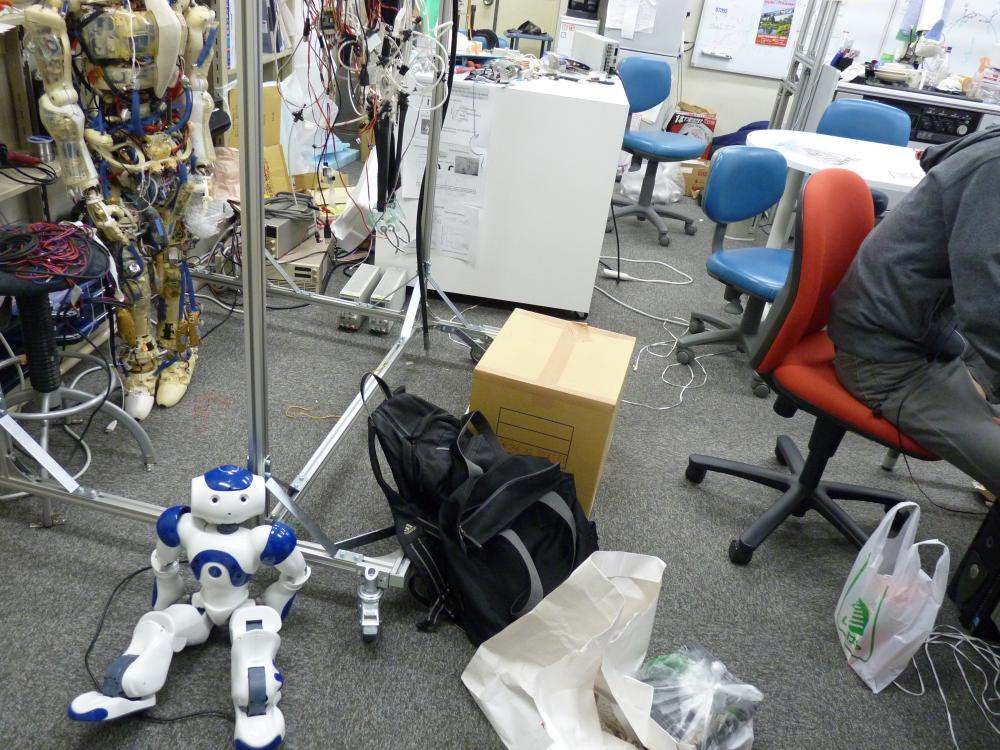
\includegraphics[width=0.50\hsize]{\FIGDIR/photo.jpg}%
    \caption{図の貼り方}%
    \label{fig:lab}%
  \end{center}%
\end{figure}%
図\ref{fig:lab}はこのようにして貼られた図である.
図に対して言及するときはこのようにrefコマンドを使う.
refコマンドの引数を,図を貼った時のコマンド群中のlabelコマンドの引数と対応させることで,意図した図に対してrefすることができるのである.

さて,先ほどの図の貼り方はちょっとめんどくさい.
大体,たかが図を一枚貼るためにこんな数行使った処理をいちいち書いてられないし,ソースコードのスペース的にもたくさん消費してしまってアホみたいである.
そのあたりを解決するのが,figコマンドである.
(figコマンドはいわば自作関数で,ikuo.styの中に定義されている.)
figコマンドを使うと,下記のように図を貼ることができる.
\fig{photo.jpg}{width=.50\hsize}{figコマンドを使って貼った図}
\figref{photo.jpg}はfigコマンドを使って貼った図である.
そして,今,気づいただろうか.
今のrefはただのrefではなく,figrefコマンドを使ってrefを行ったものである.
(figrefコマンドもfigコマンド同様にikuo.styの中で定義されている.)
figrefコマンドを使うと,いちいち「図」とか「fig.」とかをrefコマンドの前に書く必用がなくなり,便利である.
更に,「図」でなく「fig.」として参照するように変更する必用が生じた時にも,ikuo.styの中のfigrefコマンドの定義箇所にて変更をするだけで文書全体に変更が行われるのでとても有用であり,figrefコマンドを使わないのは愚かしい行為である.


\subsection{figに関連する便利コマンド}

figコマンドには残念ながら,図の位置を指定する引数が存在しない.
figコマンドの定義を見ると,位置指定オプションは[tbp]となっており,ページ上端,下端,まるまる1ページ,という優先度で位置が指定されることがわかる.
どうしてもページ下端に図を貼りたいんだ,という時にはfigbコマンドが用意されている.
\figb{photo2.jpg}{width=.50\hsize}{figbコマンドを使って貼った図}
\figref{photo2.jpg}はfigbコマンドを使って貼った図である.

どうしても位置を自分で指定したい,という場合はfigposコマンドを使う.
figposコマンドは第4引数が位置指定オプションに反映されるため,下記のように使うことができる.
\figpos{photo3.jpg}{width=.50\hsize}{figposコマンドを使って貼った図}{t}
\figref{photo3.jpg}はfigposコマンドを使って貼った図である.

上記各コマンドと合わせ,定義されているfig関連のコマンドを以下にまとめておく.
\begin{itemize}
\item fig\\
  図を貼るときに使う一番基本的なコマンド.
  位置指定は[tbp]となる.
  
\item twofigs\\
  2枚の図を立てに並べて貼るときに使うコマンド.
  キャプションは1つだけつき,ラベルは最初の図のファイル名になる.
  位置指定は[tbp]となる.
  
\item figthroug\\
  複数段組の文書中で,段組をぶちぬいて図を貼るときに使うコマンド.
  
\item figb\\
  ページ下端に図を貼るときに使うコマンド.
  
\item figpos\\
  任意の位置を指定して図を貼るときに使うコマンド.
  
\item doublefig\\
  2枚の図を横に並べて貼るときに使うコマンド.
  キャプションは1つだけつき,ラベルは最初の図のファイル名になる.
  位置指定は[tb]となる.
  
\item doublefigt\\
  doublefigコマンドと同様だが,ページ上端に図を貼るとき専用のコマンド.
  具体的には図の上側にスペースを入れずに貼ることができる.
  
\item doublefigb
  doublefigコマンドと同様だが,ページ下端に図を貼るとき専用のコマンド.
  
\item doublefigthrough\\
  doublefigコマンドと同様だが,複数段組の文章中で段組をぶちぬいて図を貼るときに使うコマンド.
  位置指定は[t]となる.
  
\item triplefig\\
  3枚の図を横に並べて貼るときに使うコマンド.
  キャプションは1つだけ表示され,ラベルは最初の図のファイル名になる.
  位置指定は[tbp]となる.
  
\item triplefigthrough\\
  triplefigコマンドと同様だが,複数段組の文章中で段組をぶちぬいて図を貼るときに使うコマンド.
  位置指定は[tbp]となる.
  
\end{itemize}


\section{表と式の書き方}
\seclabel{table_equation}

\subsection{表の書き方}
表を書くときには以下のようにする.
\begin{table}[tb]
  \label{sample}
  \begin{center}
    \caption{各人データ}
    \begin{tabular}{l|c|c|r}
      \hline
      名前 & 身長[cm] & 体重[kg] & 備考 \\
      \hline
      Y.M & 1800 & 60 & \\
      Y.M & 170 & 10 & \\
      Y.M & 170 & 60 & はげ\\
      \hline
    \end{tabular}
  \end{center}
\end{table}
表\ref{sample}は最も基本的な表の書き方の例である.
ソースコードを見ればわかる通り,この中ではlabelコマンドが使われているのだが,より便利なコマンドとしてtablabelが用意されている.
tablabelコマンドは表に対するラベルであるという情報をを自動的に付与してくれるため,これを用いることで図や式に対するラベルとごっちゃになるという問題を防ぐことができる.
同様のコマンドとしてfiglabel(図に対するラベル),equlabel(式に対するラベル),chaplabel(章に対するラベル),seclabel(節に対するラベル),subseclabel(小節に対するラベル)などが存在するので使うと良い.
\secref{fig}において用いたfigだとかtwofigだとかいった便利コマンドにおいてはその中でfiglabelが使用されている.

tablabelコマンドを用いた表は以下のようになる.
\begin{table}[tb]
  \tablabel{sample2}
  \begin{center}
    \caption{各人データ}
    \begin{tabular}{l|c|c|r}
      \hline
      名前 & 身長[cm] & 体重[kg] & 備考 \\
      \hline
      Y.M & 1800 & 60 & \\
      Y.M & 170 & 10 & \\
      Y.M & 170 & 60 & はげ\\
      \hline
    \end{tabular}
  \end{center}
\end{table}
\tabref{sample2}のようにtablabelを用いて表を書くと,tabrefコマンドを使うのが便利になる.
tabrefコマンドはfigrefコマンドのように自動で「図」とか「table」とかをつけてくれる便利コマンドである.

表に関しては特にこれ以上ローカルなコマンドとかないので,あとは研究室wikiを見るなりネットで情報探すなりして自分の書きたい表を書けるようになってください.


\subsection{式の書き方}
式は例えば以下のように書く.
\begin{eqnarray}
  \equlabel{hoge}
  hoge=hage
\end{eqnarray}

式に関してここで述べるべきことは表に関するそれとほぼ同様であり,つまりequlabelおよびequrefを使うべきであるという点のみである.
\equref{hoge}はequlabelを使ってラベル付されており,本文章冒頭のrefはequrefを用いて行われている.
式の書き方に関するそれ以外の情報は研究室wikiなりネット上で情報探すなりしてください.

\addcontentsline{toc}{chapter}{謝辞}
\markboth{謝辞}{謝辞}
% \chapter*{謝辞}
ここに謝辞を書く。
まだ書いてないうちは、\verb+\chapter*{謝辞}
ここに謝辞を書く。
まだ書いてないうちは、\verb+\chapter*{謝辞}
ここに謝辞を書く。
まだ書いてないうちは、\verb+\include{thanks}+をコメントアウトしておき
ましょう。
\begin{verbatim}
%% \addcontentsline{toc}{chapter}{謝辞}
%% \markboth{謝辞}{謝辞}
%% \include{thanks}
\end{verbatim}

emacs の人は、M-x comment-region ですね。
コメント解除は、C-u M-x comment-region ですね。

+をコメントアウトしておき
ましょう。
\begin{verbatim}
%% \addcontentsline{toc}{chapter}{謝辞}
%% \markboth{謝辞}{謝辞}
%% \chapter*{謝辞}
ここに謝辞を書く。
まだ書いてないうちは、\verb+\include{thanks}+をコメントアウトしておき
ましょう。
\begin{verbatim}
%% \addcontentsline{toc}{chapter}{謝辞}
%% \markboth{謝辞}{謝辞}
%% \include{thanks}
\end{verbatim}

emacs の人は、M-x comment-region ですね。
コメント解除は、C-u M-x comment-region ですね。


\end{verbatim}

emacs の人は、M-x comment-region ですね。
コメント解除は、C-u M-x comment-region ですね。

+をコメントアウトしておき
ましょう。
\begin{verbatim}
%% \addcontentsline{toc}{chapter}{謝辞}
%% \markboth{謝辞}{謝辞}
%% \chapter*{謝辞}
ここに謝辞を書く。
まだ書いてないうちは、\verb+\chapter*{謝辞}
ここに謝辞を書く。
まだ書いてないうちは、\verb+\include{thanks}+をコメントアウトしておき
ましょう。
\begin{verbatim}
%% \addcontentsline{toc}{chapter}{謝辞}
%% \markboth{謝辞}{謝辞}
%% \include{thanks}
\end{verbatim}

emacs の人は、M-x comment-region ですね。
コメント解除は、C-u M-x comment-region ですね。

+をコメントアウトしておき
ましょう。
\begin{verbatim}
%% \addcontentsline{toc}{chapter}{謝辞}
%% \markboth{謝辞}{謝辞}
%% \chapter*{謝辞}
ここに謝辞を書く。
まだ書いてないうちは、\verb+\include{thanks}+をコメントアウトしておき
ましょう。
\begin{verbatim}
%% \addcontentsline{toc}{chapter}{謝辞}
%% \markboth{謝辞}{謝辞}
%% \include{thanks}
\end{verbatim}

emacs の人は、M-x comment-region ですね。
コメント解除は、C-u M-x comment-region ですね。


\end{verbatim}

emacs の人は、M-x comment-region ですね。
コメント解除は、C-u M-x comment-region ですね。


\end{verbatim}

emacs の人は、M-x comment-region ですね。
コメント解除は、C-u M-x comment-region ですね。



\addcontentsline{toc}{chapter}{参考文献}
\markboth{参考文献}{参考文献}
\bibliographystyle{junsrt}
\bibliography{reference}

\end{document}
